\documentclass{article}

\usepackage{graphicx}
\usepackage{tikz}
\usepackage{tikzsymbols}
\usetikzlibrary{calc,patterns,shapes.geometric}
\pagestyle{empty}
\usepackage[margin=0pt]{geometry}
\geometry{papersize={14in,12in}}

\def\centerarc[#1](#2)(#3:#4:#5){\draw[#1] ($(#2)+({#5*cos(#3)},{#5*sin(#3)})$) arc (#3:#4:#5);}

\begin{document}
	\begin{figure}
		\centering
		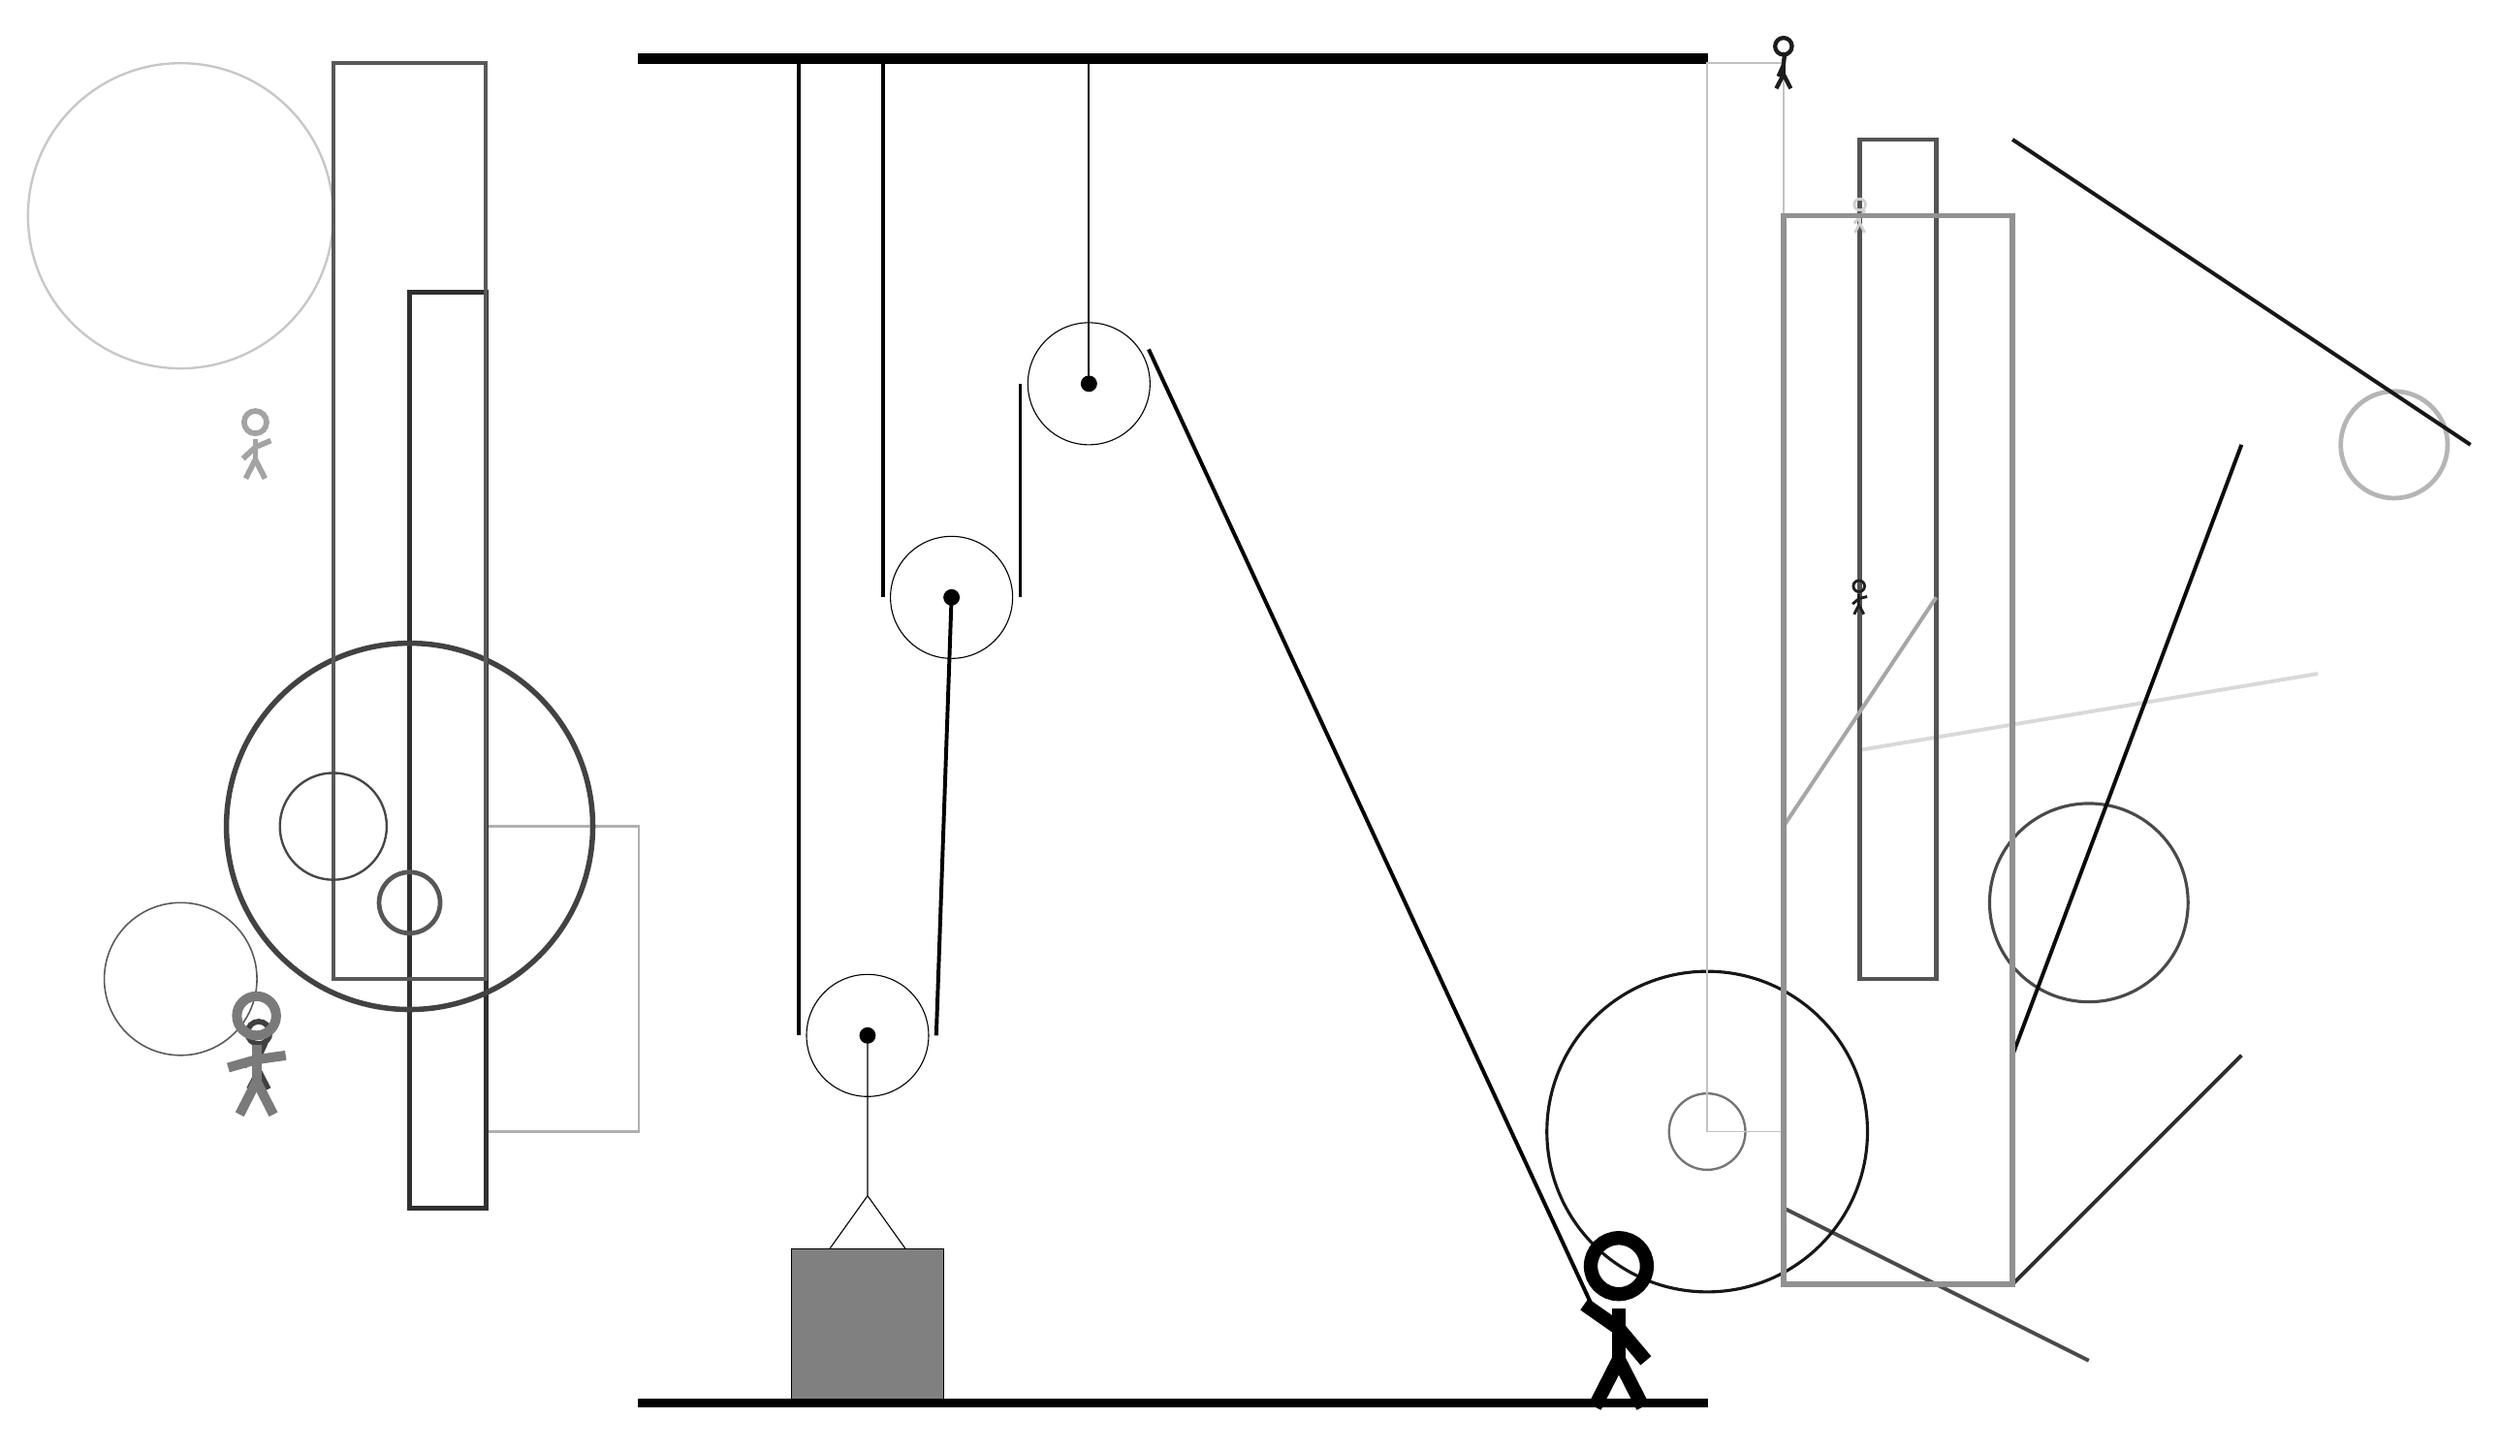
\begin{tikzpicture}
			%%%%% START %%%%%
			
			\draw[fill=black] (-2, 14) rectangle (12, 14.125);
			
			\draw (1, 1.26) circle (0.8);
			\draw[fill=black] (1, 1.26) circle (0.1);
			
			\draw[line width=0.5mm, color=black!15](14, 5) -- (20, 6);
			
			\node[line width=0.7mm, color=black!75] at (-7, 1) {\Strichmaxerl[4][29][66]};
			\draw[line width=0.3mm, color=black!31] (-4, 0) rectangle (-2, 4);
			\draw [line width=0.6mm, color=black!29](21, 9) circle (0.7);
			
			\draw[line width=0.5mm, color=black!71](17, -3) -- (13, -1);
			\draw [line width=0.3mm, color=black!22](-8, 12) circle (2.0);
			\draw[line width=0.6mm, color=black!67] (14, 2) rectangle (15, 13);
			
			\draw [line width=0.2mm, color=black!65](-8, 2) circle (1.0);
			\draw[line width=0.7mm, color=black!81] (-4, -1) rectangle (-5, 11);
			\draw[line width=0.5mm, color=black!82](16, -2) -- (19, 1);
			
			\draw [line width=0.3mm, color=black!54](12, 0) circle (0.5);
			\draw [line width=0.4mm, color=black!91](12, 0) circle (2.1);
			\draw [line width=0.4mm, color=black!71](17, 3) circle (1.3);
			\draw[line width=0.4mm, color=black!57] (-4, 11) rectangle (-4, 7);
			\node[line width=0.3mm, color=black!19] at (14, 12) {\Strichmaxerl[2][48][53]};
			\node[line width=0.2mm, color=black!88] at (14, 7) {\Strichmaxerl[2][40][14]};
			\node[line width=0.2mm, color=black!36] at (-7, 9) {\Strichmaxerl[4][43][23]};
			\node[line width=0.7mm, color=black!52] at (-7, 1) {\Strichmaxerl[7][16][8]};
			\draw[line width=0.5mm, color=black!35](13, 4) -- (15, 7);
			
			\draw[line width=0.2mm, color=black!24] (13, 14) rectangle (12, 0);
			\draw [line width=0.7mm, color=black!74](-5, 4) circle (2.4);
			
			\draw[line width=0.4mm, color=black!46] (13, -2) rectangle (15, -2);
			
			\draw [line width=0.6mm, color=black!66](-5, 3) circle (0.4);
			\draw[line width=0.5mm, color=black!96](16, 1) -- (19, 9);
			\draw[line width=0.5mm, color=black!91](16, 13) -- (22, 9);
			
			\draw[line width=0.5mm, color=black!65] (-4, 14) rectangle (-6, 2);
			\draw[line width=0.7mm, color=black!43] (13, -2) rectangle (16, 12);
			\draw [line width=0.3mm, color=black!72](-6, 4) circle (0.7);
			
			\node[line width=0.7mm, color=black!89] at (13, 14) {\Strichmaxerl[3][66][84]};
			
			\draw (2.1, 7.0) circle (0.8);
			\draw[fill=black] (2.1, 7.0) circle (0.1);
			
			\draw (3.9, 9.8) circle (0.8);
			\draw[fill=black] (3.9, 9.8) circle (0.1);
			\draw[thick] (3.9, 9.8) -- (3.9, 14);
			
			\draw (1, 1.26) -- (1, -0.84) -- (0.5, -1.54) -- (1.5, -1.54) -- (1, -0.84);
			\draw[fill=black!50] (0, -1.54) rectangle (2, -3.54);
			
			\draw[line width=0.5mm] (0.1, 14) -- (0.1, 1.26);
			\centerarc[line width=0.5mm](1, 1.26)(180:360:0.9);
			\draw[line width=0.5mm](1.9, 1.26) -- (2.1, 7.0);
			\draw[line width=0.5mm] (1.2, 14) -- (1.2, 7.0);
			\centerarc[line width=0.5mm](2.1, 7.0)(180:360:0.9);
			\draw[line width=0.5mm](3.0, 7.0) -- (3.0, 9.8);
			\centerarc[line width=0.5mm](3.9, 9.8)(30:180:0.9);
			\draw[line width=0.5mm] (4.683, 10.25) -- (10.5, -2.3);
			
			\node at (10.8, -2.5) {\Strichmaxerl[10][-35][-50]};
			
			\draw[fill=black] (-2, -3.5) rectangle (12, -3.6);
			
			%%%%% END %%%%%
		\end{tikzpicture}
	\end{figure}	
\end{document}